% This is "sig-alternate.tex" V2.0 May 2012
% This file should be compiled with V2.5 of "sig-alternate.cls" May 2012
%
% This example file demonstrates the use of the 'sig-alternate.cls'
% V2.5 LaTeX2e document class file. It is for those submitting
% articles to ACM Conference Proceedings WHO DO NOT WISH TO
% STRICTLY ADHERE TO THE SIGS (PUBS-BOARD-ENDORSED) STYLE.
% The 'sig-alternate.cls' file will produce a similar-looking,
% albeit, 'tighter' paper resulting in, invariably, fewer pages.
%
% ----------------------------------------------------------------------------------------------------------------
% This .tex file (and associated .cls V2.5) produces:
%       1) The Permission Statement
%       2) The Conference (location) Info information
%       3) The Copyright Line with ACM data
%       4) NO page numbers
%
% as against the acm_proc_article-sp.cls file which
% DOES NOT produce 1) thru' 3) above.
%
% Using 'sig-alternate.cls' you have control, however, from within
% the source .tex file, over both the CopyrightYear
% (defaulted to 200X) and the ACM Copyright Data
% (defaulted to X-XXXXX-XX-X/XX/XX).
% e.g.
% \CopyrightYear{2007} will cause 2007 to appear in the copyright line.
% \crdata{0-12345-67-8/90/12} will cause 0-12345-67-8/90/12 to appear in the copyright line.
%
% ---------------------------------------------------------------------------------------------------------------
% This .tex source is an example which *does* use
% the .bib file (from which the .bbl file % is produced).
% REMEMBER HOWEVER: After having produced the .bbl file,
% and prior to final submission, you *NEED* to 'insert'
% your .bbl file into your source .tex file so as to provide
% ONE 'self-contained' source file.
%
% ================= IF YOU HAVE QUESTIONS =======================
% Questions regarding the SIGS styles, SIGS policies and
% procedures, Conferences etc. should be sent to
% Adrienne Griscti (griscti@acm.org)
%
% Technical questions _only_ to
% Gerald Murray (murray@hq.acm.org)
% ===============================================================
%
% For tracking purposes - this is V2.0 - May 2012

\documentclass{sig-alternate}

\usepackage{graphicx}
\usepackage{datetime}
\newdateformat{mydate}{\THEDAY\ \monthname[\THEMONTH]\ \THEYEAR}

% arara: pdflatex 
% arara: bibtex 
% arara: pdflatex 
% arara: pdflatex 
\begin{document}

%
% --- Author Metadata here ---

\conferenceinfo{Data for Good Exchange 2015,}{New York, NY}

% \CopyrightYear{2007} % Allows default copyright year (20XX) to be over-ridden - IF NEED BE.
% \crdata{0-12345-67-8/90/01}  % Allows default copyright data (0-89791-88-6/97/05) to be over-ridden - IF NEED BE.
% --- End of Author Metadata ---

\title{Pushing Data Science Education into the Real World}
% \subtitle{xxxxxx}

%
% You need the command \numberofauthors to handle the 'placement
% and alignment' of the authors beneath the title.
%
% For aesthetic reasons, we recommend 'three authors at a time'
% i.e. three 'name/affiliation blocks' be placed beneath the title.
%
% NOTE: You are NOT restricted in how many 'rows' of
% "name/affiliations" may appear. We just ask that you restrict
% the number of 'columns' to three.
%
% Because of the available 'opening page real-estate'
% we ask you to refrain from putting more than six authors
% (two rows with three columns) beneath the article title.
% More than six makes the first-page appear very cluttered indeed.
%
% Use the \alignauthor commands to handle the names
% and affiliations for an 'aesthetic maximum' of six authors.
% Add names, affiliations, addresses for
% the seventh etc. author(s) as the argument for the
% \additionalauthors command.
% These 'additional authors' will be output/set for you
% without further effort on your part as the last section in
% the body of your article BEFORE References or any Appendices.

\numberofauthors{3}
%  in this sample file, there are a *total*
% of EIGHT authors. SIX appear on the 'first-page' (for formatting
% reasons) and the remaining two appear in the \additionalauthors section.
%
\author{
% You can go ahead and credit any number of authors here,
% e.g. one 'row of three' or two rows (consisting of one row of three
% and a second row of one, two or three).
%
% The command \alignauthor (no curly braces needed) should
% precede each author name, affiliation/snail-mail address and
% e-mail address. Additionally, tag each line of
% affiliation/address with \affaddr, and tag the
% e-mail address with \email.
%
% 1st. author
\alignauthor
Daniel Turek\\
       \affaddr{\small{Berkeley Institute for Data Science}}\\
       \affaddr{\small{University of California, Berkeley}}\\
       \affaddr{\small{190 Doe Library, Berkeley, CA}}\\
       \email{\normalsize{\texttt{anthonysuen@berkeley.edu}}}
% 2nd. author
\alignauthor
Anthony Suen\\
       \affaddr{\small{Berkeley Institute for Data Science}}\\
       \affaddr{\small{University of California, Berkeley}}\\
       \affaddr{\small{190 Doe Library, Berkeley, CA}}\\
       \email{\normalsize{\texttt{dturek@berkeley.edu}}}
% 3rd. author
\alignauthor
Dav Clark\\
       \affaddr{\small{Berkeley Institute for Data Science}}\\
       \affaddr{\small{University of California, Berkeley}}\\
       \affaddr{\small{190 Doe Library, Berkeley, CA}}\\
       \email{\normalsize{\texttt{davclark@berkeley.edu}}}
}

% \date{30 July 1999}
\date{\mydate\today}


% A category with the (minimum) three required fields
% \category{H.4}{Information Systems Applications}{Miscellaneous}
% A category including the fourth, optional field follows...
% \category{D.2.8}{Software Engineering}{Metrics}[complexity measures, performance measures]
% \terms{Theory}
% \keywords{ACM proceedings, \LaTeX, text tagging}


\maketitle

\begin{abstract}

The discipline of data science has been viewed as an convergence of high-power computing, data visualization and analysis, and data-driven application domains over the past decade.  Prominent research institutions and private sector industry have been quick to embrace the importance of data science, but the foundations for effective tertiary-level data science education are conspicuously absent. This is nothing new, however, as the university has a well-established tradition of developing its educational mission hand in hand with the development of novel methods for human understanding \cite{feingold_tradition_1991}. Thus it is natural that universities "figure out" data science hand in hand with the development of needed pedagogy. We consider the development of data science education with respect to recent trends in interdisciplinary and experiential education, along with agile and design thinking methodologies to understand how they could apply to data science educational programs. This historical perspective motivates us to consider what factors are necessary to drive effective data science education, which range from a complete end-to-end workflow, technological tools for development and team communications, and appropriate motivation and incentives. The first iteration of the \emph{Berkeley Institute for Data Science (BIDS) Collaborative} started in the University of California, Berkeley in the Spring of 2015 is used as a case study. From this we draw lessons learned and form a hypothesis regarding the necessary ingredients for effective data science education at the tertiary level ? a topic that is presently understudied.  This hypothesis will be tested and revised in subsequent iterations of the BIDS Collaborative as we continue our study of effective data science education, research, and social impact.

\end{abstract}

\section{Introduction}

The rapid advances in computational power and the on-going "big data" craze, the discipline of data science has exploded onto the academic and business landscape. Master's programs in data science are now being offered at premier research institutions such as Stanford University and Columbia University, and centers for data science have recently opened their doors at the University of California, Berkeley, the University of Washington, and New York University. Led  by the success of tech giants such as Google, Amazon and Facebook, the increasing availability of data is transforming industries ranging from medicine to media.  The industrial sector is keeping pace by creating and actively recruiting for positions in data science.  The profession of data scientist was even described by the Harvard Business Review as "the sexiest job of the 21$^{\text{st}}$ century" \cite{Patil2012}.

Despite this inundation of the term "data science," we still struggle to define what data science is, or to realise any boundaries as to what data science encompasses \cite{Hayashi1998, Loukides2011, Provost2013}. A common Venn diagram places data science squarely at the intersection of computer science, mathematical statistics, and scientific application domains.  This perhaps most accurately depicts that data science is nebulous by nature, having ties to all areas of quantitative scientific research or computational data analysis, but falls short of providing an understanding of how this new scientific discipline will eventually settle into the scientific ecosystem.  Fortunately, our aim is not to pin down the nature of data science itself, but instead to examine the practicalities and realities of data science education at the tertiary level.

There exists substantial literature regarding best practices and modern approaches to tertiary education. This has been a subject of interest since the first modern Universities appeared in Europe \cite{Rudy1984, Pedersen1997}.  Since then, the approach to higher education has evolved immensely, due to advances in technology, and also society's attitude towards higher education.  Perhaps the single-most transformative influence on higher education has been the so-called digital revolution of the past decades, which has had a profound impact on the content and style of tertiary education \cite{Roberts1994, Ely1995, Baker1997, Wood2005, Baek2008}.

Some research suggests that traditional approaches to tertiary education may only result in superficial learning, rather than a deep understanding of subject material \cite{Entwistle1992}.  Thus, the study of education itself is an area of prime interest.  Many approaches have been suggested and studied over the past decades, in attempts to improve education at the tertiary level.  \cite{Topping1996} promotes the practice of peer-tutoring, while others have more recently endorsed "flipped classrooms" in which learning becomes more self-directed (as opposed to instructor-directed) and classrooms become a place for practice instead of lecture \cite{Horn2013, Herreid2013}.  \cite{Ogawa1995} suggests a "mutiscience" approach to multidisciplinary science education, in which the diversity scientific disciplines is recognized and incorporated into the educational system.  Project-based learning has been promoted at the institutional level for many years \cite{Krajcik2006, Thomas2000}.

We re-focus our attention to the fledgling field of data science, but now in the context of education.  In light of the academic and industry spotlight on data science, experiences  and best practices for data science education should be a prime focus of research, just as it is for tertiary education in general.  However, owing to its relatively recent mainstream debut, there is a noteworthy absence of scientific research or published literature on the subject of data science education.  This fact motivates our present analysis of the history, current trends, and future prospects of data science education.

We aim to begin filling this void by providing a tangible case study of data science education, which was undertaken at the University of California, Berkeley, under the BIDS Collaborative. We consider the successes and failures of the first cohort to pass through the Collaborative, and the pain points which were encountered by the students and mentors, alike.  We make practical recommendations for educational approaches to data science curricula, and formulate a hypothesis regarding the "best practices" of tertiary data science education.  Study of our hypothesis will require subsequent experiential testing, which will be the subject of  on-going and future research.



\section{Case Study: \\BIDS Collaborative}

As detailed above, the central organizing principle of the collaborative was to organize teams of students around data science projects. In standard data science education, a common concern is the selection of domain-appropriate materials that will be of interest given a student's background. Thus, one of our primary concerns was to ensure projects that would be of interest to a wide variety of students, and we therefore collected a large, diverse set spanning 16 projects. 

Based on lessons learned at the DSSG program in Chicago, we requested that project clients have data ready in hand that they were able to share with student teams. We also attempted to ensure that projects were clearly framed as an answerable question (though as we will discuss below, most projects were more exploratory, and this was not a bad thing). It seems clear in hindsight, however, that student enthusiasm for a project was driven almost entirely by the presence of the "client" to give a pitch to students during one of two informational sessions at the beginning of the semester. Given limited time and resources for managing the collaborative, most client proposals were not vetted for data availability. Ultimately, four projects received enough interest, along with a project from a team that had already formed prior to their participation in the collaborative (these projects are detailed below).

\subsection{Project Selection and Team Formation}

The BIDS Collaborative ran five projects during the course of the semester, with clients from industry, academia, non-profit, and government. Details of specific projects are relayed in separate sections below. Each project took a somewhat idiosyncratic course, though there were clear commonalities, both in terms of challenges and solutions. Teams consisting of four members from various disciplines were suggested. A particular concern was the need to balance teams so not everyone was technical.

Team formation was somewhat chaotic and arguably the most difficult part of the process from the facilitator perspective. Participants were largely attracted via two "mixers" at the beginning of the Spring 2015 semester, which consisted of a brief motivational presentation after which we asked students to meet with one another and form teams around one of the available projects. Students were given a large number of choices, and were encouraged to organize themselves via a google spreadsheet. While self-organization might work more efficiently via a system that could enforce a set of rules and policies, allowing all students to collaboratively edit a spreadsheet created numerous problems. The most dramatic difficulty occurred when a large number of student responses were inadvertently deleted from the spreadsheet. Ultimately, our efforts to create a "self-service" approach required facilitators in the collaborative (the authors of this paper) to engage in a very time-intensive process, organizing teams via extensive conversations in person and via email. While attendance at the mixers was quite strong, the collaborative ultimately retained thirteen individuals from the initial cohort, with an additional three joining a few weeks into the semester. One individual dropped off mid-semester (this individual was actually staff at Lawrence Berkeley National Labs, and not a student), though participation was otherwise stable after the first few weeks of the spring semester.

An additional challenge at the beginning of the Spring 2015 semester was the lack of leadership in the various teams. Teams could best be described as loose assemblies of individuals working relatively independently on related topics, and progress was slow. Recognizing this lack of cohesion, we suggested that each team choose a lead -- a process that generally consisted of one person volunteering to take on this role. At least one individual expressed reluctance to engage in a management role, as their interest was largely in hands-on experience \emph{doing data science}. Moreover, after this transition, it was often difficult for these reluctant managers to lead their teams.  At this stage, team leads served a gatekeeper function in allowing students into their team. For these students, the authority of the team lead appeared to be more established. To be clear, "authority" here was very gently exercised, and primarily consisted of working with facilitators to be clear about intended work, and progress achieved. 

Given the above lessons, In the upcoming Fall 2015 session, we intend to focus on identifying clear team leads for a set of projects. At this point, facilitators can work with team leads to select remaining team members. This will serve to simplify and distribute the process of team formation, while also clearly establishing a leadership role for the team lead from the beginning.

\subsection{Projects}

\begin{figure*}
\centerline{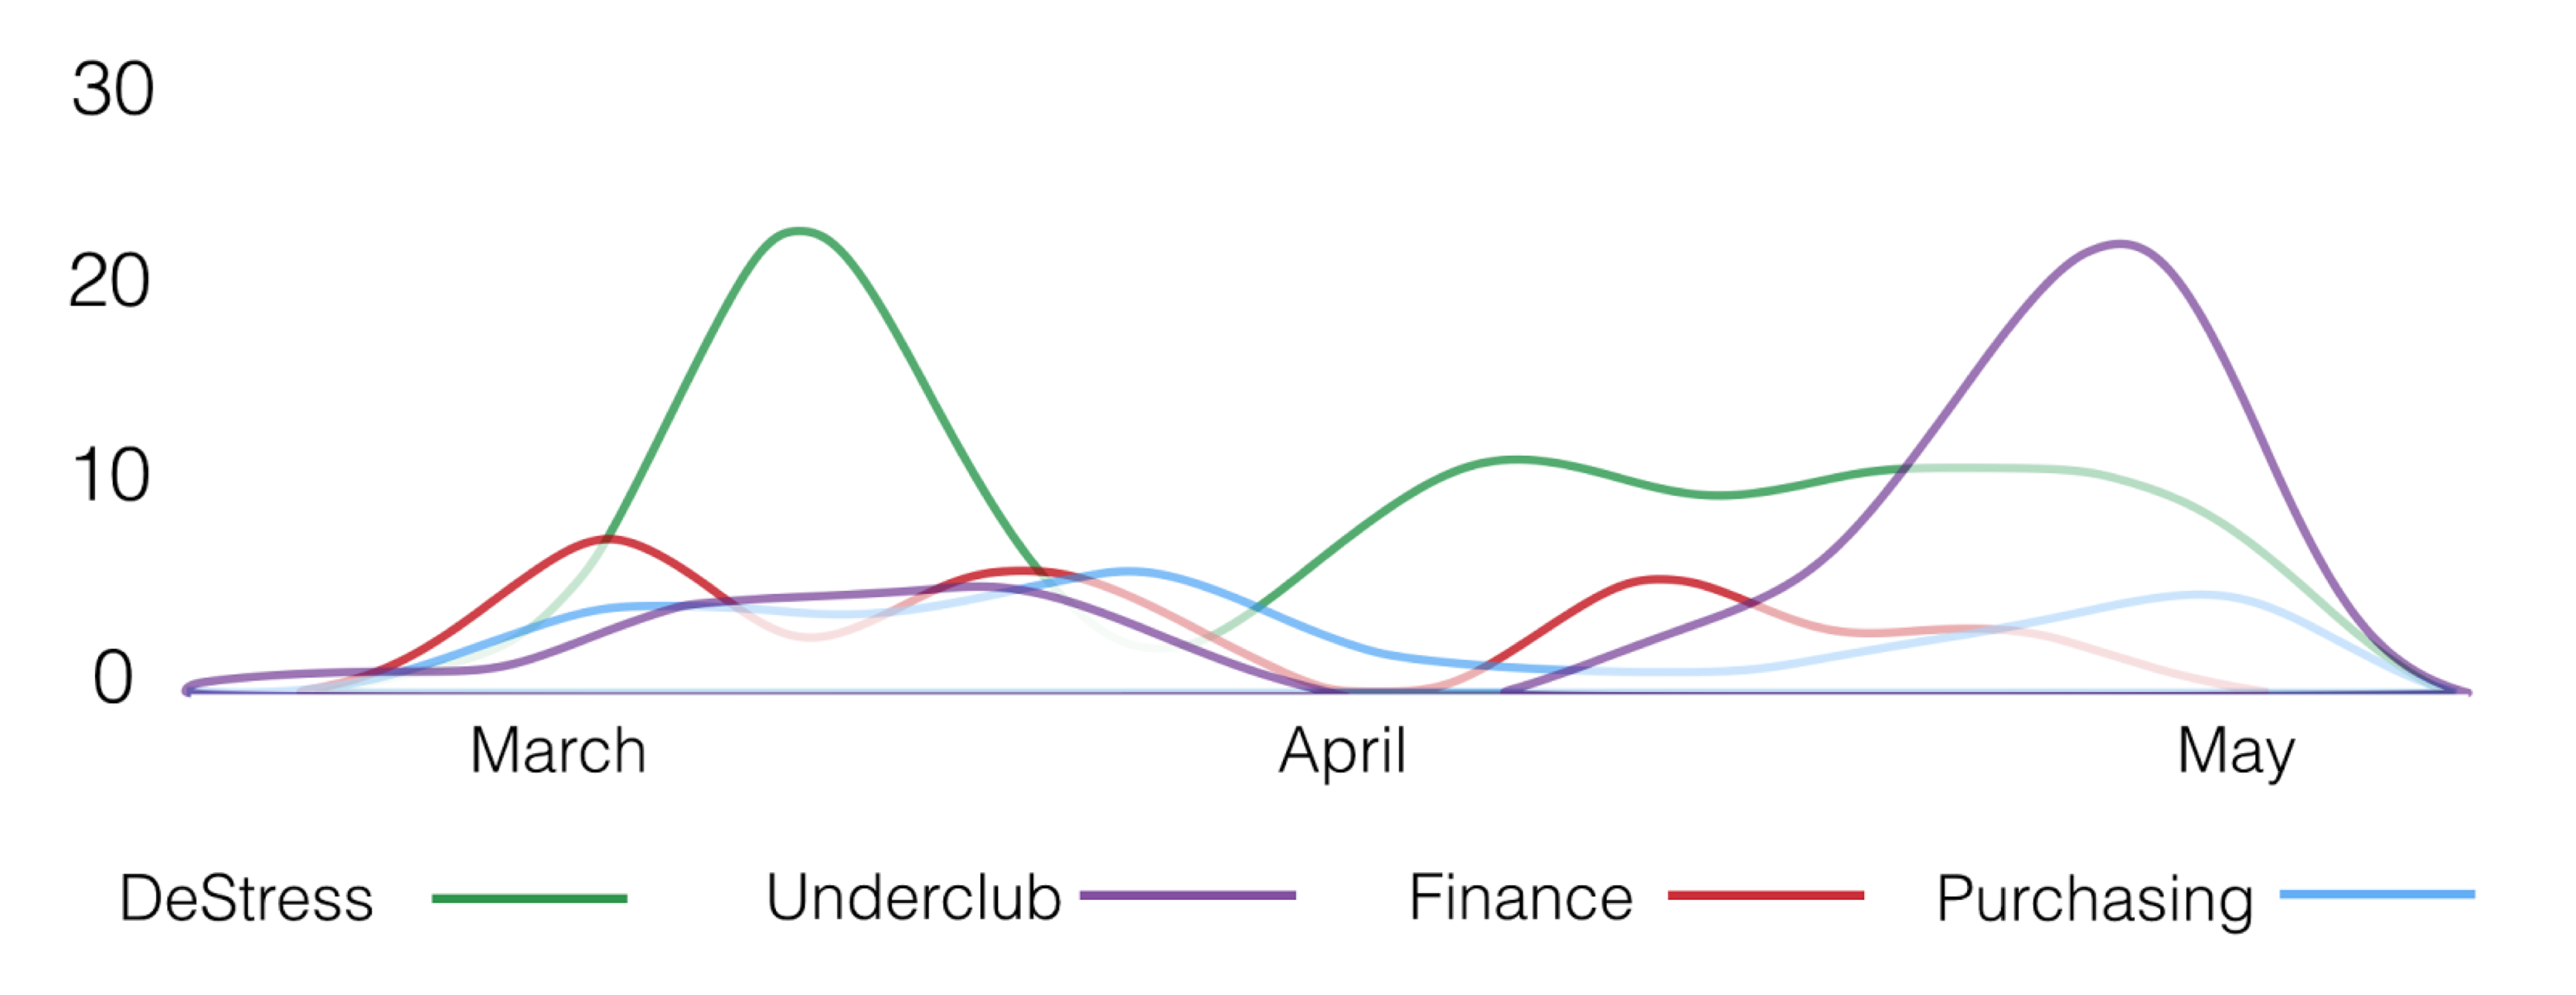
\includegraphics[scale=0.27]{dsc_figure_gitcommits.png}}
\caption{History of GitHub commits made by each BIDS Collaborative project team between March and May 2015.}
\label{fig:gitcommits}
\end{figure*}

While both the facilitators and participating teams were divided on the issue at first, all teams switched to development on GitHub in a matter of weeks. Teams formed in mid-February, and all teams were committing to GitHub by March (Figure~\ref{fig:gitcommits}). While a training on collaborative software development with GitHub was provided in the context of "The Hacker Within" meeting in BIDS, few members of the collaborative were able to attend. The differing skill-levels of the participants further problematized training in these skills. As such, the start was a bit rocky, and again consisted primarily of smaller-scale coaching from facilitators and mentors. Relatedly, the usage of BIDS space was ad hoc, with some members of the BIDS community finding this usage disruptive. This was addressed by identifying a single weekday where collaborative members were particularly encouraged to attend and "take over" the space, and to be particularly conscientious (for example, using private breakout rooms) outside of this time.

In our upcoming session, we have thus adopted a clear plan that we will establish immediately at the beginning of the semester. Students will be encouraged to come to a practicum on a weekday that will include an initial half-hour of orientation to technical tooling, including project management and documentation.


\subsubsection*{Strategic Sourcing}

Director of the University of California's strategic sourcing unit had a pre-existing connection with the Berkeley D-Lab (\texttt{http://dlab.berkeley.edu/}), primarily via a previous analyst's use of D-Lab python training and consulting. This work led to a conference talk at SciPy 2014 discussing how straightforward scientific python scripts were able to accelerate previously spreadsheet-based analyses from taking approximately a week to a matter of minutes. A Collaborative facilitator assisted strategic sourcing in this work, and was therefore well aware of the opportunities available to save the university system time and money. From the perspective of an academic institution, this project illustrates an exciting double-win, with potential benefits to administration and student training. 

We learned from this attempt that it is incredibly hard for a team of graduate students to obtain actionable insights while working only a few hours per week for a semester. Useful progress was made, however, in identifying basic workflows and determining which questions appear to be answerable. In particular, clustering techniques showed promise in identifying non-obvious partnerships where collective purchasing might provide savings.

Another key insight that five hours was insufficient to maintain consistent progress, as much time is spent each week keep track of what happened. Ten hours seems to be required at a minimum. 


\subsubsection*{Text Mining for Stress}

This was one of two projects that was actually driven by faculty involvement. What differentiated these projects from standard faculty-driven research was the inclusive call for participation, and the engagement in a collaborative open-source development framework. In this case, we pursued a project using Prof. John Canny's BIDMach system (\cite{canny2013bidmach}; \texttt{http://bid2.berkeley.edu/bid-data-project/}), a performant GPU-accelerated system for machine learning in the Scala language. A domain focus on determining stress and major life events using large-scale machine learning was chosen by one of Prof. Canny's graduate students, Pablo Paredes.

The project was enabled in part by providing a commodity workstation (with GPU) that was already available in the D-Lab, with the addition 1TB of hard disk storage. Thus, while this project was pushing the limits of academic machine learning, the resources for this project would be readily accessible to modestly funded labs. This project maintains robust activity, and the participants are working towards the publication of a handful of papers this summer.


\subsubsection*{Analyzing Financial Market Data with Spark}

This project was the second of two that was driven by a faculty member, in this case, Prof. Justin McCrary, faculty director of the D-Lab. Prof. McCrary has been working to develop efficient workflows to take advantage of the UC Berkeley campus compute cluster, Savio. To this end, we worked with the Berkeley Research Computing team that manages the cluster to enable a modern Spark-based workflow. Unlike other projects, this initiative had large startup costs, including software installation challenges, and integrating with the traditional HPC Scheduler (Slurm). As such, much of the semester was spent getting to proof-of-concept workflows using spark to analyze a subset of the data. Despite modest progress on the domain questions, this project was likely of the highest value to campus, as it improved the ability to take advantage of the impressive parallel capabilities that are now provided to all senior campus researchers as a "birthright" -- particularly for those users who may need something other than a traditional HPC workflow.


\subsubsection*{Underclub}

While our intention was to primarily recruit clients from outside the university, Underclub was the only client that approximated this intent. Indeed, even they had a pre-existing affiliation with the university via the Haas school of business (the founder was a Haas graduate, and Underclub remains connected to the school). Much as with the strategic sourcing project above, participants struggled to achieve actionable insights, though again promising directions were established. It is clear that more guidance is needed to efficiently connect analysis with potential business-relevant actions.



%\subsection{Figures}
%Like tables, figures cannot be split across pages; the best placement for them is typically the top or the bottom of the page nearest their initial mention.  To ensure this proper ``floating'' placement of figures, use the environment \textbf{figure} to enclose the figure and its caption.
%
%This sample document contains examples of \textbf{.eps} and \textbf{.ps} files to be displayable with \LaTeX.  More details on each of these is found in the \textit{Author's Guide}.
%
%\begin{figure}[h]
%\centerline{\includegraphics[scale=1.0]{FIGNAME}}
%\caption{CAPTION}
%\label{LABEL}
%\end{figure}
% 
%\begin{figure}
%\centering
%\epsfig{file=fly.eps}
%\caption{A sample black and white graphic (.eps format).}
%\end{figure}
%
%\begin{figure}
%\centering
%\epsfig{file=fly.eps, height=1in, width=1in}
%\caption{A sample black and white graphic (.eps format)
%that has been resized with the \texttt{epsfig} command.}
%\end{figure}
%
%As was the case with tables, you may want a figure that spans two columns.  To do this, and still to ensure proper ``floating'' placement of tables, use the environment \textbf{figure*} to enclose the figure and its caption. and don't forget to end the environment with {figure*}, not {figure}!
%
%\begin{figure*}
%\centering
%\epsfig{file=flies.eps}
%\caption{A sample black and white graphic (.eps format)
%that needs to span two columns of text.}
%\end{figure*}
%
%Note that either {\textbf{.ps}} or {\textbf{.eps}} formats are used; use the \texttt{{\char'134}epsfig} or \texttt{{\char'134}psfig} commands as appropriate for the different file types.
%
%\begin{figure}
%\centering
%\psfig{file=rosette.ps, height=1in, width=1in,}
%\caption{A sample black and white graphic (.ps format) that has
%been resized with the \texttt{psfig} command.}
%\vskip -6pt
%\end{figure}



%ACKNOWLEDGMENTS are optional

%\section{Acknowledgments}
%This section is optional; it is a location for you to acknowledge grants, funding, editing assistance and what have you.  In the present case, for example, the authors would like to thank Gerald Murray of ACM for his help in codifying this \textit{Author's Guide} and the \textbf{.cls} and \textbf{.tex} files that it describes.



% The following two commands are all you need in the
% initial runs of your .tex file to
% produce the bibliography for the citations in your paper.

\bibliographystyle{abbrv}
% \bibliography{sigproc}    % sigproc.bib is the name of the Bibliography in this case
\bibliography{ZoteroLibrary,davs-lone-reference}



% You must have a proper ".bib" file
%  and remember to run:
% latex bibtex latex latex
% to resolve all references
%
% ACM needs 'a single self-contained file'!



%%APPENDICES are optional

%%\balancecolumns
%\appendix
%%Appendix A
%\section{Headings in Appendices}
%The rules about hierarchical headings discussed above for
%the body of the article are different in the appendices.
%In the \textbf{appendix} environment, the command
%\textbf{section} is used to
%indicate the start of each Appendix, with alphabetic order
%designation (i.e. the first is A, the second B, etc.) and
%a title (if you include one).  So, if you need
%hierarchical structure
%\textit{within} an Appendix, start with \textbf{subsection} as the
%highest level. Here is an outline of the body of this
%document in Appendix-appropriate form:
%\subsection{Introduction}
%\subsection{The Body of the Paper}
%\subsubsection{Type Changes and  Special Characters}
%\subsubsection{Math Equations}
%\paragraph{Inline (In-text) Equations}
%\paragraph{Display Equations}
%\subsubsection{Citations}
%\subsubsection{Tables}
%\subsubsection{Figures}
%\subsubsection{Theorem-like Constructs}
%\subsubsection*{A Caveat for the \TeX\ Expert}
%\subsection{Conclusions}
%\subsection{Acknowledgments}
%\subsection{Additional Authors}
%This section is inserted by \LaTeX; you do not insert it.
%You just add the names and information in the
%\texttt{{\char'134}additionalauthors} command at the start
%of the document.
%\subsection{References}
%Generated by bibtex from your ~.bib file.  Run latex,
%then bibtex, then latex twice (to resolve references)
%to create the ~.bbl file.  Insert that ~.bbl file into
%the .tex source file and comment out
%the command \texttt{{\char'134}thebibliography}.
%% This next section command marks the start of
%% Appendix B, and does not continue the present hierarchy
%\section{More Help for the Hardy}
%The sig-alternate.cls file itself is chock-full of succinct
%and helpful comments.  If you consider yourself a moderately
%experienced to expert user of \LaTeX, you may find reading
%it useful but please remember not to change it.
%%\balancecolumns % GM June 2007
%% That's all folks!



\end{document}
